\begin{question}[ID=1.1, subtitle={Satellite in orbita circolare con periodo di 24 ore}, tags={moto circolare, satellite}, difficulty=media]
Un satellite orbita intorno alla Terra in un'orbita circolare di raggio $r = 7{,}5\times10^6\ \mathrm{m}$ compiendo un giro in $24\ \mathrm{ore}$.
\begin{enumerate}
\item Determina il periodo in secondi.
\item Determina la frequenza di rotazione.
\item Calcola la velocità tangenziale.
\item Trova l'accelerazione centripeta.
\end{enumerate}
\begin{solution}
\begin{enumerate}
\item Il periodo è il tempo di un giro completo, convertito in secondi: $T = 24\cdot 3600 = 86\,400\ \mathrm{s}$.
\item La frequenza è il numero di giri al secondo, cioè l'inverso del periodo: $f = 1/T \approx 1{,}16\times10^{-5}\ \mathrm{Hz}$.
\item La velocità tangenziale è la lunghezza dell'orbita ($2\pi r$) divisa per il periodo:
\[
v = \frac{2\pi r}{T} = \frac{2\pi\cdot 7{,}5\times10^6}{86\,400} \approx \mathbf{545\ \mathrm{m/s}}.
\]
\item L'accelerazione centripeta, diretta verso il centro, vale $a_c = v^2/r$:
\[
a_c = \frac{v^2}{r} = \frac{545^2}{7{,}5\times10^6} \approx \mathbf{0{,}0397\ \mathrm{m/s^2}}.
\]
\end{enumerate}
\end{solution}
\end{question}

%------------------------------------------------------------------------------------%

\begin{question}[ID=1.2, subtitle={Stazione Spaziale Internazionale — velocità e forza centripeta}, tags={moto circolare, satellite}, difficulty=media]
L'ISS di massa $419\,455\ \mathrm{kg}$ orbita a $r = 6700\ \mathrm{km}$ con periodo $T = 92{,}7\ \mathrm{min}$.
\begin{enumerate}
\item Calcola il periodo in secondi.
\item Calcola la velocità tangenziale.
\item Calcola la forza centripeta che subisce l'ISS.
\end{enumerate}
\begin{solution}
\begin{enumerate}
\item Convertiamo il periodo in secondi: $T = 92{,}7\cdot 60 = 5562\ \mathrm{s}$.
\item La velocità tangenziale è il perimetro dell'orbita diviso il periodo:
\[
v = \frac{2\pi r}{T} = \frac{2\pi\cdot 6{,}7\times10^6}{5562} \approx \mathbf{7565\ \mathrm{m/s}}.
\]
\item La forza centripeta è quella che mantiene l'ISS in orbita, $F_c = m a_c = mv^2/r$:
\[
F_c = \frac{mv^2}{r} = \frac{419\,455\cdot 7565^2}{6{,}7\times10^6} \approx \mathbf{3{,}58\times10^6\ \mathrm{N}}.
\]
\end{enumerate}
\end{solution}
\end{question}

%------------------------------------------------------------------------------------%

\begin{question}[ID=1.3, subtitle={Centrifuga per insalata — periodo, velocità e accelerazione centripeta}, tags={moto circolare}, difficulty=media]
\begin{minipage}{\linewidth}
\begin{wrapfigure}{r}{0.25\textwidth}
    \centering
    \vspace{-30pt}
    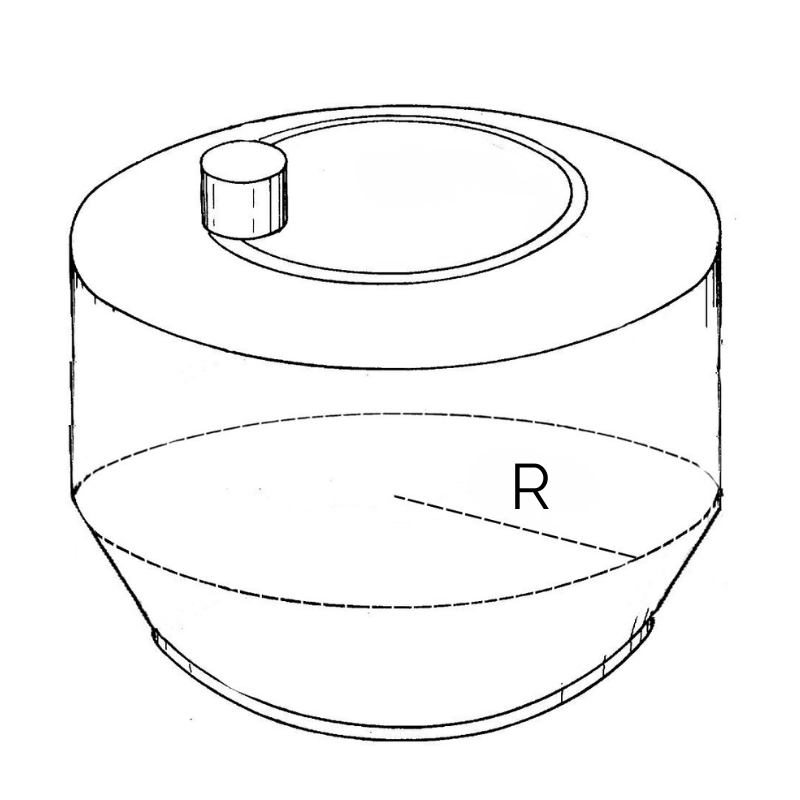
\includegraphics[width=0.25\textwidth]{images/salad_spinner.png}
\end{wrapfigure}
Una centrifuga per insalata ha raggio $R = 25\ \mathrm{cm}$ e ruota $3$ volte al secondo.
\begin{enumerate}[parsep=0pt,itemsep=2pt]
\item Calcola il periodo di rotazione.
\item Calcola la velocità tangenziale e angolare.
\item Calcola l'accelerazione centripeta di una goccia sulla parete.
\end{enumerate}
\end{minipage}
\begin{solution}
\begin{enumerate}
\item Il periodo è l'inverso della frequenza ($f = 3\ \mathrm{Hz}$): $T = 1/f = 1/3 \approx 0{,}333\ \mathrm{s}$.
\item La velocità angolare è $\omega = 2\pi f$ e quella tangenziale $v = \omega R$:
\[
\omega = 2\pi f = 6\pi \approx 18{,}85\ \mathrm{rad/s}, \qquad v = \omega R = 18{,}85\cdot 0{,}25 \approx \mathbf{4{,}71\ \mathrm{m/s}}.
\]
\item L'accelerazione centripeta che «schiaccia» la goccia contro la parete è $a_c = \omega^2 R$:
\[
a_c = \omega^2 R = (6\pi)^2\cdot 0{,}25 = 9\pi^2 \approx \mathbf{88{,}8\ \mathrm{m/s^2}}.
\]
\end{enumerate}
\end{solution}
\end{question}

%------------------------------------------------------------------------------------%

\begin{question}[ID=1.4, subtitle={Disco che ruota a 250 giri/min — angolo descritto in 0,1 s}, tags={moto circolare, velocità angolare}, difficulty=facile]
Un disco ruota attorno a un asse passante per il centro e compie $250\ \mathrm{giri/min}$.
\begin{enumerate}
\item Quanti radianti descrive un punto del disco in $0{,}1\ \mathrm{s}$?
\item La risposta dipende dalla distanza del punto dall'asse?
\end{enumerate}
\begin{solution}
\begin{enumerate}
\item Convertiamo la frequenza in velocità angolare ($\omega = 2\pi\cdot\text{giri al secondo}$); l'angolo descritto nel moto uniforme è $\theta = \omega t$:
\[
\omega = \frac{250\cdot 2\pi}{60} = 26{,}18\ \mathrm{rad/s}, \qquad \theta = \omega\,t = 26{,}18\cdot 0{,}1 \approx \mathbf{2{,}62\ \mathrm{rad}}.
\]
\item \textbf{No}: la velocità angolare $\omega$ è la stessa per tutti i punti del disco rigido, quindi tutti descrivono lo stesso angolo, indipendentemente dalla distanza dall'asse (ciò che cambia è la velocità tangenziale $v = \omega r$).
\end{enumerate}
\end{solution}
\end{question}

%------------------------------------------------------------------------------------%

\begin{question}[ID=1.5, subtitle={Orologio — velocità e accelerazione centripeta delle tre lancette}, tags={moto circolare}, difficulty=media]
Un orologio ha lancetta delle ore lunga $1\ \mathrm{cm}$, dei minuti $1{,}4\ \mathrm{cm}$ e dei secondi $1{,}6\ \mathrm{cm}$.
\begin{enumerate}
\item Calcola il periodo di ogni punto estremo.
\item Calcola la velocità angolare e tangenziale dei tre punti.
\item Calcola le rispettive accelerazioni centripete.
\end{enumerate}
\begin{solution}
Ogni lancetta percorre un giro completo in un tempo diverso (12 h, 1 h, 1 min); da $T$ si ricavano $\omega = 2\pi/T$, $v = \omega r$ e $a_c = \omega^2 r$. Riassumendo i risultati per i tre punti estremi:
\begin{tabular}{lccc}
 & Ore & Minuti & Secondi \\
\hline
$T$ & $43\,200\ \mathrm{s}$ & $3600\ \mathrm{s}$ & $60\ \mathrm{s}$ \\
$\omega\ (\mathrm{rad/s})$ & $1{,}45\times10^{-4}$ & $1{,}75\times10^{-3}$ & $0{,}1047$ \\
$v\ (\mathrm{m/s})$ & $1{,}45\times10^{-6}$ & $2{,}44\times10^{-5}$ & $1{,}68\times10^{-3}$ \\
$a_c\ (\mathrm{m/s^2})$ & $2{,}1\times10^{-10}$ & $4{,}3\times10^{-8}$ & $1{,}76\times10^{-4}$ \\
\end{tabular}

Si nota come la lancetta dei secondi, pur essendo solo poco più lunga, abbia velocità e accelerazione enormemente maggiori, perché ruota molto più rapidamente.
\end{solution}
\end{question}

%------------------------------------------------------------------------------------%

\begin{question}[ID=1.6, subtitle={Satellite TV geostazionario a 36000 km di quota}, tags={moto circolare, satellite}, difficulty=media]
Un satellite TV è a quota $h = 36\,000\ \mathrm{km}$, periodo $T = 24\ \mathrm{h}$. $R_{Terra} = 6370\ \mathrm{km}$.
\begin{enumerate}
\item Calcola la velocità angolare.
\item Calcola la velocità tangenziale.
\item Calcola l'accelerazione centripeta.
\end{enumerate}
\begin{solution}
Il raggio dell'orbita si misura dal centro della Terra, quindi somma il raggio terrestre e la quota: $r = 6370 + 36\,000 = 42\,370\ \mathrm{km} = 4{,}237\times10^7\ \mathrm{m}$.
\begin{enumerate}
\item La velocità angolare dipende solo dal periodo: $\omega = 2\pi/T = 2\pi/86\,400 \approx 7{,}27\times10^{-5}\ \mathrm{rad/s}$.
\item La velocità tangenziale è $v = \omega r \approx \mathbf{3081\ \mathrm{m/s}}$.
\item L'accelerazione centripeta è $a_c = \omega^2 r \approx \mathbf{0{,}224\ \mathrm{m/s^2}}$.
\end{enumerate}
\end{solution}
\end{question}

%------------------------------------------------------------------------------------%

\begin{question}[ID=1.7, subtitle={Lavatrice a 500 giri/min — accelerazione centripeta della biancheria}, tags={moto circolare}, difficulty=facile]
Il cestello di una lavatrice ha diametro $40\ \mathrm{cm}$ e ruota a $500\ \mathrm{giri/min}$.
\begin{enumerate}
\item Calcola l'accelerazione centripeta della biancheria.
\end{enumerate}
\begin{solution}
Il raggio è metà del diametro ($r = 0{,}20\ \mathrm{m}$) e la velocità angolare si ottiene convertendo i giri al minuto in rad/s ($\omega = 500\cdot 2\pi/60 = 52{,}36\ \mathrm{rad/s}$). L'accelerazione centripeta è allora
\[
a_c = \omega^2 r = 52{,}36^2\cdot 0{,}20 \approx \mathbf{548\ \mathrm{m/s^2}} \approx 56\,g.
\]
È questo valore elevatissimo, decine di volte $g$, a strizzare l'acqua dalla biancheria.
\end{solution}
\end{question}

%------------------------------------------------------------------------------------%

\begin{question}[ID=1.8, subtitle={Ruota di bicicletta — giri, frequenza e angolo}, tags={moto circolare}, difficulty=media]
Una ruota di bicicletta ha diametro $40\ \mathrm{cm}$ e velocità tangenziale $v = 1{,}4\ \mathrm{m/s}$.
\begin{enumerate}
\item Quanti giri compie in $2\ \mathrm{min}$?
\item Con quale frequenza gira?
\item Qual è l'angolo descritto dalla valvola in $0{,}2\ \mathrm{s}$?
\end{enumerate}
\begin{solution}
Dalla velocità tangenziale ricaviamo velocità angolare e periodo: $\omega = v/r = 1{,}4/0{,}20 = 7\ \mathrm{rad/s}$ e $T = 2\pi/\omega = 0{,}898\ \mathrm{s}$.
\begin{enumerate}
\item In $2\ \mathrm{min} = 120\ \mathrm{s}$ il numero di giri è il tempo diviso il periodo: $n = 120/T \approx \mathbf{133{,}7\ \mathrm{giri}}$.
\item La frequenza è l'inverso del periodo: $f = 1/T \approx \mathbf{1{,}11\ \mathrm{Hz}}$.
\item L'angolo descritto nel moto uniforme è $\theta = \omega t = 7\cdot 0{,}2 = \mathbf{1{,}4\ \mathrm{rad}}$.
\end{enumerate}
\end{solution}
\end{question}

%------------------------------------------------------------------------------------%

\begin{question}[ID=1.9, subtitle={Titano — luna di Saturno: velocità angolare, tangenziale e centripeta}, tags={moto circolare, satellite}, difficulty=media]
Titano orbita a $r = 1\,222\,000\ \mathrm{km}$ con periodo $T = 15\ \mathrm{d}\ 23\ \mathrm{h}$.
\begin{enumerate}
\item Calcola la velocità angolare.
\item Calcola la velocità tangenziale.
\item Calcola l'accelerazione centripeta.
\item Calcola la frequenza in Hz.
\end{enumerate}
\begin{solution}
Convertiamo periodo e raggio in unità SI: $T = (15\cdot 24 + 23)\cdot 3600 = 1\,378\,800\ \mathrm{s}$ e $r = 1{,}222\times10^9\ \mathrm{m}$.
\begin{enumerate}
\item Velocità angolare: $\omega = 2\pi/T \approx 4{,}56\times10^{-6}\ \mathrm{rad/s}$.
\item Velocità tangenziale: $v = \omega r \approx \mathbf{5569\ \mathrm{m/s}}$.
\item Accelerazione centripeta: $a_c = \omega^2 r \approx \mathbf{0{,}0254\ \mathrm{m/s^2}}$.
\item Frequenza: $f = \omega/(2\pi) \approx 7{,}26\times10^{-7}\ \mathrm{Hz}$ (un'orbita ogni 16 giorni circa).
\end{enumerate}
\end{solution}
\end{question}

%------------------------------------------------------------------------------------%

\begin{question}[ID=1.10, subtitle={Corpo con frequenza 10 Hz — angolo descritto in 1 s}, tags={moto circolare, velocità angolare}, difficulty=facile]
Un corpo gira con frequenza $f = 10\ \mathrm{Hz}$.
\begin{enumerate}
\item Quale angolo descrive il raggio in $1\ \mathrm{s}$?
\end{enumerate}
\begin{solution}
La velocità angolare è $\omega = 2\pi f = 20\pi\ \mathrm{rad/s}$ e nel moto uniforme l'angolo cresce come $\theta = \omega t$:
\[
\theta = \omega t = 20\pi\cdot 1 = \mathbf{20\pi \approx 62{,}8\ \mathrm{rad}}.
\]
Equivale a 10 giri completi, coerentemente con una frequenza di 10 Hz mantenuta per un secondo.
\end{solution}
\end{question}

%------------------------------------------------------------------------------------%

\begin{question}[ID=1.11, subtitle={Punto su traiettoria circolare con ω = 2,4 rad/s}, tags={moto circolare, velocità angolare}, difficulty=facile]
Un punto mobile descrive una traiettoria circolare di raggio $r = 12\ \mathrm{cm}$ con velocità angolare costante $\omega = 2{,}4\ \mathrm{rad/s}$.
\begin{enumerate}
\item Calcola la frequenza del moto.
\item Calcola la velocità tangenziale.
\end{enumerate}
\begin{solution}
\begin{enumerate}
\item La frequenza si ottiene dalla velocità angolare dividendo per $2\pi$: $f = \omega/(2\pi) = 2{,}4/(2\pi) \approx \mathbf{0{,}382\ \mathrm{Hz}}$.
\item La velocità tangenziale è il prodotto della velocità angolare per il raggio: $v = \omega r = 2{,}4\cdot 0{,}12 = \mathbf{0{,}288\ \mathrm{m/s}}$.
\end{enumerate}
\end{solution}
\end{question}

%------------------------------------------------------------------------------------%

\begin{question}[ID=1.12, subtitle={Pallina su cerchio con accelerazione centripeta 5 m/s²}, tags={moto circolare, accelerazione centripeta}, difficulty=media]
Una pallina gira su una circonferenza di raggio $r = 20\ \mathrm{cm}$ con accelerazione centripeta $a_c = 5\ \mathrm{m/s^2}$.
\begin{enumerate}
\item Calcola la velocità tangenziale.
\item Calcola il periodo.
\item Calcola la frequenza.
\item Calcola la velocità angolare.
\end{enumerate}
\begin{solution}
\begin{enumerate}
\item Invertendo $a_c = v^2/r$ ricaviamo la velocità tangenziale: $v = \sqrt{a_c\,r} = \sqrt{5\cdot 0{,}20} = \mathbf{1\ \mathrm{m/s}}$.
\item Il periodo è il perimetro diviso la velocità: $T = 2\pi r/v = 2\pi\cdot 0{,}20/1 \approx \mathbf{1{,}257\ \mathrm{s}}$.
\item La frequenza è l'inverso del periodo: $f = 1/T \approx \mathbf{0{,}795\ \mathrm{Hz}}$.
\item La velocità angolare è $\omega = v/r = 1/0{,}20 = \mathbf{5\ \mathrm{rad/s}}$.
\end{enumerate}
\end{solution}
\end{question}

%------------------------------------------------------------------------------------%

\begin{question}[ID=1.13, subtitle={Velocità tangenziale e accelerazione centripeta all'equatore terrestre}, tags={moto circolare, Terra}, difficulty=media]
Il raggio medio della Terra è $R = 6370\ \mathrm{km}$; un giro completo in $T = 24\ \mathrm{h}$.
\begin{enumerate}
\item Calcola la velocità tangenziale di un punto all'equatore.
\item Calcola l'accelerazione centripeta dello stesso punto.
\end{enumerate}
\begin{solution}
\begin{enumerate}
\item Un punto all'equatore percorre l'intera circonferenza terrestre in un giorno, quindi $v = 2\pi R/T$:
\[
v = \frac{2\pi\cdot 6{,}37\times10^6}{86\,400} \approx \mathbf{463\ \mathrm{m/s}}.
\]
\item L'accelerazione centripeta è $a_c = v^2/R$:
\[
a_c = \frac{463^2}{6{,}37\times10^6} \approx \mathbf{0{,}0337\ \mathrm{m/s^2}},
\]
piccolissima rispetto a $g$: per questo la rotazione terrestre influisce solo lievemente sul peso apparente.
\end{enumerate}
\end{solution}
\end{question}


%====================================================%
% FAC
%====================================================%
\begin{question}[ID=fac, subtitle={Sovrapposizione delle lancette in 12 ore}, tags={moto circolare}, difficulty=difficile]
\textbf{FAC)} Quante volte si sovrappongono le lancette delle ore e dei minuti in 12 ore, e a che orari?
\begin{solution}
La lancetta dei minuti compie 1 giro/h, quella delle ore 1/12 giro/h. Le due si sovrappongono quando l'angolo percorso in più dalla lancetta dei minuti è un numero intero di giri:
\[
\frac{t}{60} - \frac{t}{720} = k \;\Rightarrow\; t = \frac{720k}{11}\ \text{minuti}, \quad k = 0,1,2,\ldots,10.
\]
In 12 ore si hanno quindi $\mathbf{11}$ sovrapposizioni (i casi $k = 0$ e $k = 11$ coincidono entrambi a mezzanotte/mezzogiorno).

Orari approssimativi: 12:00, 1:05, 2:11, 3:16, 4:22, 5:27, 6:33, 7:38, 8:44, 9:49, 10:55.
\end{solution}
\end{question}
